%%%%%%%%%%%%%%%%%%%%%%%%%%%%%%%%%%%%%%%%%
% Beamer Presentation
% LaTeX Template
% Version 1.0 (10/11/12)
%
% This template has been downloaded from:
% http://www.LaTeXTemplates.com
%
% License:
% CC BY-NC-SA 3.0 (http://creativecommons.org/licenses/by-nc-sa/3.0/)
%
%%%%%%%%%%%%%%%%%%%%%%%%%%%%%%%%%%%%%%%%%

%----------------------------------------------------------------------------------------
%	PACKAGES AND THEMES
%----------------------------------------------------------------------------------------

\documentclass{beamer}
\usepackage{subcaption}

\mode<presentation> {

% The Beamer class comes with a number of default slide themes
% which change the colors and layouts of slides. Below this is a list
% of all the themes, uncomment each in turn to see what they look like.

%\usetheme{default}
%\usetheme{AnnArbor}
%\usetheme{Antibes}
%\usetheme{Bergen}
%\usetheme{Berkeley}
%\usetheme{Berlin}
%\usetheme{Boadilla}
%\usetheme{CambridgeUS}
%\usetheme{Copenhagen}
%\usetheme{Darmstadt}
%\usetheme{Dresden}
%\usetheme{Frankfurt}
%\usetheme{Goettingen}
%\usetheme{Hannover}
%\usetheme{Ilmenau}
%\usetheme{JuanLesPins}
%\usetheme{Luebeck}
\usetheme{Madrid}
%\usetheme{Malmoe}
%\usetheme{Marburg}
%\usetheme{Montpellier}
%\usetheme{PaloAlto}
%\usetheme{Pittsburgh}
%\usetheme{Rochester}
%\usetheme{Singapore}
%\usetheme{Szeged}
%\usetheme{Warsaw}

% As well as themes, the Beamer class has a number of color themes
% for any slide theme. Uncomment each of these in turn to see how it
% changes the colors of your current slide theme.

%\usecolortheme{albatross}
%\usecolortheme{beaver}
%\usecolortheme{beetle}
%\usecolortheme{crane}
%\usecolortheme{dolphin}
%\usecolortheme{dove}
%\usecolortheme{fly}
%\usecolortheme{lily}
%\usecolortheme{orchid}
%\usecolortheme{rose}
%\usecolortheme{seagull}
%\usecolortheme{seahorse}
%\usecolortheme{whale}
%\usecolortheme{wolverine}

%\setbeamertemplate{footline} % To remove the footer line in all slides uncomment this line
%\setbeamertemplate{footline}[page number] % To replace the footer line in all slides with a simple slide count uncomment this line

%\setbeamertemplate{navigation symbols}{} % To remove the navigation symbols from the bottom of all slides uncomment this line
}

\usepackage{graphicx} % Allows including images
\usepackage{booktabs} % Allows the use of \toprule, \midrule and \bottomrule in tables

%----------------------------------------------------------------------------------------
%	TITLE PAGE
%----------------------------------------------------------------------------------------

\title[]{Toward an Agent-Based Simulation of the Factors Impacting Diversity within a College Student Body} % The short title appears at the bottom of every slide, the full title is only on the title page
%short title can go in the brackets

\author{Stephen Davies \inst{1} \and Morgan Brown \inst{2}} % Your name
\institute[] % Your institution as it will appear on the bottom of every slide, may be shorthand to save space
{
\inst{1} University of Mary Washington \and \inst{2} University of Wisconsin - Madison\\ % Your institution for the title page
}
\date{\today} % Date, can be changed to a custom date

\begin{document}

\begin{frame}
\titlepage % Print the title page as the first slide
\end{frame}

%\begin{frame}
%\frametitle{Overview} % Table of contents slide, comment this block out to remove it
%\tableofcontents % Throughout your presentation, if you choose to use \section{} and \subsection{} commands, these will automatically be printed on this slide as an overview of your presentation
%\end{frame}

%----------------------------------------------------------------------------------------
%	PRESENTATION SLIDES
%----------------------------------------------------------------------------------------

%------------------------------------------------
\section{Motivation} % Sections can be created in order to organize your presentation into discrete blocks, all sections and subsections are automatically printed in the table of contents as an overview of the talk
%------------------------------------------------

%\subsection{Subsection Example} % A subsection can be created just before a set of slides with a common theme to further break down your presentation into chunks

\begin{frame}
\frametitle{Motivation}
Goals:

\begin{itemize}
\itemsep.1em
\item to create a useful abstraction for the domain of \textit{peer influence
on a college campus}
\item to experiment and establish the quantitative effects and boundaries of
\textit{key parameters}
\item to \textit{validate} the model against real-world empirical data
\item to \textit{ascertain the possible effects of certain policies} that
institutions might choose to enact to encourage racial integration.
\end{itemize}

\end{frame}

%------------------------------------------------

\begin{frame}
\frametitle{The Problem}
\begin{itemize}
\item College enrollment rates for racial minorities are disproportionately
low across the United States. (Ryu 2010)
\pause
\item Attrition is consistently higher for minorities than for white students.
(Zea \textit{et al.} 1997)
\pause
\item Alienation has been identified as a key contributor to these effects,
particularly \textbf{social estrangement}. (Kao \textit{et al.} 2003, Kalsner
1991, Suen 1983)
\pause
\item ``...even if minority students show high levels of academic
satisfaction, they may feel socially and culturally alienated." (Loo 1986)
\end{itemize}

\end{frame}

%------------------------------------------------

\begin{frame}
\frametitle{Dominant factors in forming friendships}
Propinquity: The more often two people encounter one another, the more likely
it is they will form a friendship. (Mouw \textit{et al.} 2006)\\

~~\\

\pause
Homophily: People with similar traits are more likely to form friendships with
one another. (McPherson \textit{et al.} 2001)
\begin{itemize}
\item hobbies
\item values
\item personal preferences
\item race, age, gender
\end{itemize}

~~\\

\pause
Both of these factors work \textit{against} racial integration. What would
have to happen to the evolving social network of a college campus to help
foster integration?
\end{frame}

%------------------------------------------------

\begin{frame}
\frametitle{Our Approach}
The network of friendships on a college campus is the result of (among other things) the innumerable chance encounters, impressions, and choices to form relationships that have occurred over years.\\

~~\\

We describe an agent-based simulation to model these interrelationships and influences. Software objects representing individual students:
\begin{enumerate}
\item possess a set of malleable attributes and a ``race" trait;
\item encounter each other randomly;
\item decide whether or not to form friendships;
\item influence the attributes of their friends;
\item dissolve the friendships which are not ``refreshed" often enough by additional future encounters.
\end{enumerate}

~~\\
We use ``number of friendships" as a proxy for social estrangement.
\end{frame}

%------------------------------------------------

%\begin{frame}
%\frametitle{Multiple Columns}
%\begin{columns}[c] % The "c" option specifies centered vertical alignment while the "t" option is used for top vertical alignment
%
%\column{.45\textwidth} % Left column and width
%\textbf{Heading}
%\begin{enumerate}
%\item Statement
%\item Explanation
%\item Example
%\end{enumerate}
%
%\column{.5\textwidth} % Right column and width
%Lorem ipsum dolor sit amet, consectetur adipiscing elit. Integer lectus nisl, ultricies in feugiat rutrum, porttitor sit amet augue. Aliquam ut tortor mauris. Sed volutpat ante purus, quis accumsan dolor.
%
%\end{columns}
%\end{frame}

%------------------------------------------------
\section{The Model}
%------------------------------------------------

% I don't think we need this slide; it seems mostly a repeat from above.
%\begin{frame}
%\frametitle{Purpose}
%CollegeSim is an agent-based model designed to simulate an evolving social network among college students. 
%
%Student agents are assigned one of two ``races" which factors into their perceived similarity to other agents, and accordingly to their likelihood of forming friendships with them. 
%
%The ultimate goal of the model is to investigate how racial segregation is affected by the strength of the race trait and the presence or absence of certain institutional policies designed to influence segregation.
%\end{frame}

%------------------------------------------------

\begin{frame}
\frametitle{Entities, State Variables and Scales}
Two entities: Students and Groups.\\

~~\\

Each Student has the following attributes:
\begin{enumerate}
\item Race: Either ``white" or ``minority."
\item Year: An integer from 1 to 4 indicating the Student's current year in school.
\item Preferences: An array of real numbers between 0 and 1 representing the student's abstract preferences. These values are independent of one another.
\item Hobbies: An array of real numbers between 0 and 1 representing how much of the student's time is dedicated to a particular activity. These values are not independent of one another and always sum to 1.
\item Friends: An array of references to other Student objects with whom it has active relationships.
\end{enumerate}
\end{frame}

%------------------------------------------------

\begin{frame}
\frametitle{Entities, State Variables and Scales}
Groups are evolving sets of students that represent some social tie. (Members
of a common academic course or major; common party-goers; members of an
extra-curricular club; those who live on the same
dormitory floor; \textit{etc.}) 

~~\\
Each Group has the following attributes:
\begin{enumerate}
\item IsFixed: A logical value indicating whether or not the group's membership is permanently fixed.
\item RecruitmentFactor: A real number between 0 and 1 indicating how aggressive the group is in attracting new members.
\item Members: An array of references to the Students who comprise its membership.
\end{enumerate}
\end{frame}

%------------------------------------------------

\begin{frame}
\frametitle{Process Overview and Scheduling}
Each academic year consists of nine academic months and three summer months. Student and Group agents carry out actions in each academic month. A high-level controller carries out actions at the beginning and end of each academic year.\\

\begin{enumerate}
\item At the start of each academic year, new student agents (freshmen) and
new social groups are created.
\item In each academic month, each Student randomly encounters other students,
adjusts their attributes due to their friends' influence, and discontinues old
friendships.
\item In each academic month, each Group influences its members, recruits new
students, and loses some students. 
\item At the end of each academic year, seniors graduate.
\end{enumerate}
\end{frame}

%------------------------------------------------

\begin{frame}
\frametitle{Some interesting model parameters}

\begin{enumerate}
\item The proportion of white students ($p_w$) in the student body

\item ``Race weight" ($w_r$) --- the importance of same-race to homophily
calculations (measured in ``equivalent number of attributes")

\item ``Decay threshold" ($t_d$) --- the number of time steps (simulated
months) at which a friendship will be dissolved if the two friends did not
encounter each other during that time (to ``refresh")

\item Monthly group encounters ($n_{eg}$) --- the number of students from
his/her groups that each student encounters monthly

\item Monthly population encounters ($n_{ep}$) --- the number of students from
the overall population that each student encounters monthly

\end{enumerate}

\end{frame}

%------------------------------------------------
\begin{frame}
\frametitle{Experimental policies}

\begin{enumerate}

\item \textbf{Force initial biracial friendships.} When enabled, each Student
is initially provided with $n_{d0}$ friendships of randomly selected other
students of the opposite race.

\item \textbf{Orientation groups.} When enabled, $n_{f0}$ \textit{fixed}
groups are created in addition to the other groups. Students are deliberately
assigned so that the proportion of minorities is higher in groups with
minorities.

\end{enumerate}

In both cases, the goal is to combat segregation by mandating exposure to
opposite-race peers early in a student's career.

~~\\

Question: to what degree can policies like these influence the degree of social
integration of minorities?
\end{frame}

%------------------------------------------------

% I think these is TMI, and should be described more generally (as it was
% above.)
%\begin{frame}
%\frametitle{Submodels}
%\begin{enumerate}
%\item IncrementYears: Add 1 to the Year attribute of every Student still in the simulation.
%\item AddNewStudents: Add new Student agents to the simulation with unique IDs, Year = 1, and set probability of being white. Each of some number of Preferences and Hobbies are generated and then hobbies are normalized so that they sum to 1.
%\item AddNewGroups: Some number of Groups are created with unique IDs and with isFixed equal to FALSE. Each Group is randomly assigned initial students. Each Group's RecruitmentFactor is generated.
%\item ComputeSimilarity: Given two Student agents, compute their perceived similarity.
%\item ComputeAffinity: Given a Student and a Group, compute the mean similarity between the Student and all individual members of the Group.
%\end{enumerate}
%\end{frame}
%
%%------------------------------------------------
%
%\begin{frame}
%\frametitle{Submodels}
%\begin{enumerate}
%\item EncounterOthers: Choose some number of other students at random from the Student's current Groups and some other number from the population at large. For each one, if the two Students are already friends, ``refresh" their friendship. If not, determine the Students' similarity via the ComputeSimilarity submodel and compute their probability of becoming friends. With this probability, make the two Students friends.
%\item AdjustAttributes: For each of a Student's preferences and hobbies, compute the average value of that preference/hobby for all friends of that Student. Then, with some probability, adjust the Student's attribute towards the mean by some coefficient multipled by the difference between its current value and the mean.
%\item InfluenceMembers: Adjust the attribute values for each Student in the Group, using the exact same algorithm as the AdjustAttributes submodel except that instead of using the Students' friends' mean, use the Group members' mean.
%\end{enumerate}
%\end{frame}
%
%%------------------------------------------------
%
%\begin{frame}
%\frametitle{Submodels}
%\begin{enumerate}
%\item DecayFriendships: Remove the friendship with each of the Student's friends who has not been ``refreshed" in the most recent academic months.
%\item RecruitStudents: Choose some number of Students from the general population and compute their affinity to this Group via ComputeAffinity. For each of the Students who are not already a member of the Group, compute the probability of joining the group.
%\item GraduateStudents: Remove every Student with Year = 4 from the simulation.
%\end{enumerate}
%\end{frame}

%------------------------------------------------
\section{Preliminary Validation}
%------------------------------------------------

\begin{frame}
\frametitle{Simulation Verification}
Consider the average number of friends held by minorities and whites across
all years to verify that social estrangement is impacted:

\begin{table}[htb]
\centering
\caption{For varying race weights, the average number of friends that 
students have during senior year.\label{friendshipsVsRaceWeight}}
\begin{tabular}{|c|c|c|c|}
\hline
$w_r$ & Whites & Minorities  & $p$-value\\
\hline
0 & 15.66 & 15.73 & 0.0784\\
10 & 15.54 & 14.15 & $<2.2\times 10^{-16}$\\
20 & 15.49 & 12.97 & $<2.2\times 10^{-16}$\\
100 & 15.43 & 7.90 & $<2.2\times 10^{-16}$\\
\hline
\end{tabular}
\end{table}
\end{frame}

\begin{frame}
\frametitle{Simulation Verification}
Consider the perceived similarity between students who encounter each other,
and how often that leads to friendship.

\begin{figure}
\begin{subfigure}{.45\textwidth}
  \centering
    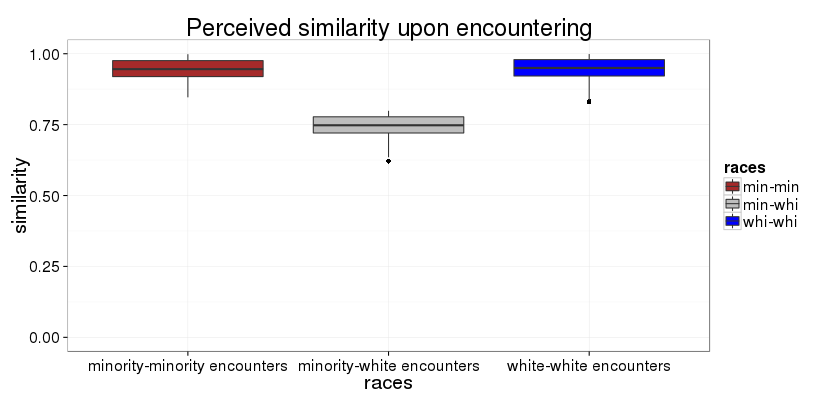
\includegraphics[width=1.2\textwidth]{similarityBoxplots20.png}
      \caption{Perceived similarity.}
\end{subfigure}
\begin{subfigure}{.45\textwidth}
    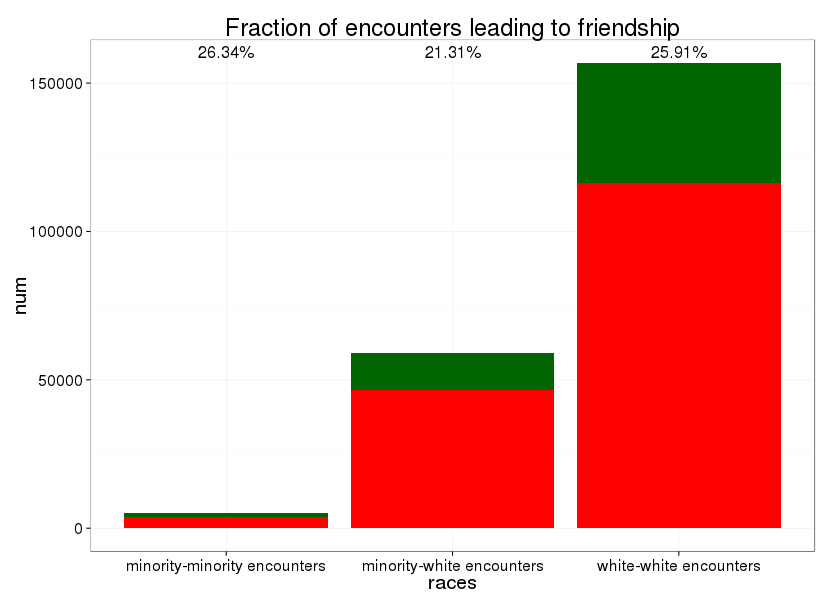
\includegraphics[width=\textwidth]{encountersGraph20.png}
      \caption{Fraction of encounters leading to friendship.}
\end{subfigure}
\caption{Perceived similarity and encounters for $w_r=20$.}
\end{figure}
\end{frame}
%------------------------------------------------

\begin{frame}
\frametitle{Discoveries}

The \textbf{Orientation Groups} policy has a significant influence on student
friendships only when $r_w$ (the race weight) and/or $n_{fo}$ (the number of
orientation groups) is quite high. 

~~\\

\pause

The \textbf{Force initial biracial friendships} policy did not have much
effect. We believe this is due to friendship decay outweighing the forced
propinquity: even if students are deliberately matched with opposite-race
students early in their college careers, those friendships will soon decay if
not refreshed often enough, which will happen if segregation is a strong
factor.

\end{frame}

%------------------------------------------------

\begin{frame}
\frametitle{Moving forward}

Our next steps with this verified and partially validated model:

~~\\

Experiment with policy parameters, especially in conjunction with one another,
to see how extreme they would have to be to combat segregation.

~~\\

Experiment with $p_w$ --- is there a ``tipping point" for the proportion of
whites beyond which the social estrangement experienced by minorities cannot
be overcome?

~~\\

Investigate the extent of attribute influence that is occurring. Is this
happening more often with whites than minorities? Is racial integration
accompanied by increased homogeneity of attributes?
\end{frame}

%------------------------------------------------

\begin{frame}
\frametitle{Acknowledgements}

Thanks to:
\begin{itemize}
\itemsep.1em
\item ACM SIGSIM and UMW Dean's Office for travel funding
\item Madeline Lord and Jessica White, UMW computer science majors
\item Dr.~Leah Cox, UMW VP of Diversity and Inclusion
\end{itemize}

\end{frame}

%\begin{frame}
%\frametitle{Table}
%\begin{table}
%\begin{tabular}{l l l}
%\toprule
%\textbf{Treatments} & \textbf{Response 1} & \textbf{Response 2}\\
%\midrule
%Treatment 1 & 0.0003262 & 0.562 \\
%Treatment 2 & 0.0015681 & 0.910 \\
%Treatment 3 & 0.0009271 & 0.296 \\
%\bottomrule
%\end{tabular}
%\caption{Table caption}
%\end{table}
%\end{frame}
%
%%------------------------------------------------
%
%\begin{frame}
%\frametitle{Theorem}
%\begin{theorem}[Mass--energy equivalence]
%$E = mc^2$
%\end{theorem}
%\end{frame}
%
%%------------------------------------------------
%
%\begin{frame}[fragile] % Need to use the fragile option when verbatim is used in the slide
%\frametitle{Verbatim}
%\begin{example}[Theorem Slide Code]
%\begin{verbatim}
%\begin{frame}
%\frametitle{Theorem}
%\begin{theorem}[Mass--energy equivalence]
%$E = mc^2$
%\end{theorem}
%\end{frame}\end{verbatim}
%\end{example}
%\end{frame}
%
%%------------------------------------------------
%
%\begin{frame}
%\frametitle{Figure}
%Uncomment the code on this slide to include your own image from the same directory as the template .TeX file.
%%\begin{figure}
%%\includegraphics[width=0.8\linewidth]{test}
%%\end{figure}
%\end{frame}
%
%%------------------------------------------------
%
%\begin{frame}[fragile] % Need to use the fragile option when verbatim is used in the slide
%\frametitle{Citation}
%An example of the \verb|\cite| command to cite within the presentation:\\~
%
%This statement requires citation \cite{p1}.
%\end{frame}
%
%%------------------------------------------------
%
%\begin{frame}
%\frametitle{References}
%\footnotesize{
%\begin{thebibliography}{99} % Beamer does not support BibTeX so references must be inserted manually as below
%\bibitem[Smith, 2012]{p1} John Smith (2012)
%\newblock Title of the publication
%\newblock \emph{Journal Name} 12(3), 45 -- 678.
%\end{thebibliography}
%}
%\end{frame}

%------------------------------------------------

\begin{frame}
\frametitle{References}

\scriptsize
\begin{itemize}
\itemsep.5em

\item Kalsner, L. (1991). Issues in College Student Retention. Higher Education
Extension Service Review, 3(1). 

\item Loo, C. M., \& Rolison, G. (1986). Alienation of Ethnic Minority Students at a
Predominantly White University. The Journal of Higher Education, 57(1), 58.

\item McPherson, M., Smith-Lovin, L., \& Cook, J. M. (2001). Birds of a feather:
Homophily in social networks. Annual Review of Sociology, 415-444.

\item Ryu, M. (2010). Minorities in Higher Education: 24th Status Report. American Council on Education.

\item Suen, H. K. (1983). Alienation and attrition of Black college students on a predominantly White campus. Journal of College Student Personnel, 24(2),
117-121.

\item Zea, M. C., Reisen, C. A., Beil, C., \& Caplan, R. D. (1997). Predicting
Intention to Remain in College Among Ethnic Minority and Nonminority Students.
The Journal of Social Psychology, 137(2), 149-160.
\end{itemize}
\end{frame}

%----------------------------------------------------------------------------------------

\end{document} 
